Qualität und Qualitätsansprüche werden meiner Ansicht nach in der heutigen Zeit 
- ungeachtet des immer noch herrschenden "`Geiz"'-Trends - wieder extrem 
wichtig und teilweise geschäftsentscheidend für viele Unternehmen. Ein großer
Teil der Konsumenten scheint wieder darauf zu achten, was man für sein Geld
eigentlich bekommt. Nebenbei steigen auch die Qualitätsansprüche an Behörden
oder öffentliche Einrichtungen. Arbeitsämter nennen sich nun "`Agentur für
Arbeit"' und wollen ihren "`Kunden"' einen besseren Service bieten. Hochschulen
stehen einer gesteigerten Erwartungshaltung der Studierenden gegenüber, die für
ihre Hochschulgebühren eine Steigerung der Lehr-Qualität erwarten.

In der vorliegenden Hausarbeit soll aufgezeigt werden, wie ein 
Qualitätsmanagementsystem (QMS) auf Basis der internationalen ISO 9001-Norm in 
einem Unternehmen eingeführt werden kann und welche Zielsetzungen es dabei 
gibt. Dazu betrachte ich ein fiktives mittelständisches Software-Unternehmen, 
dessen Hauptgeschäftsfeld die Konzeption, Entwicklung und Wartung von 
Individual-Software im Bereich Banken, Finanzdienstleister und Versicherungen 
ist.

\section{Begriffe}
In den nachfolgenden Abschnitten sollen einige zentrale Begriffe für die
Anwendung in dieser Arbeit definiert werden.

\subsection{Qualität}
Allgemein beschreibt \emph{Qualität} die Beschaffenheit, Güte oder den Wert 
einer bestimmten Sache, eines Produkts oder einer Dienstleistung. Im 
alltäglichen Sprachgebrauch ist der Begriff Qualität häufig verknüpft mit einer 
Wertung. Man spricht von "`guter"' oder "`schlechter"' Qualität.

Im Normendeutsch wird Qualität definiert als "`Grad, in dem ein Satz inhärenter 
Merkmale Anforderungen erfüllt"' \cite[S.~18]{din9000} - also als Maß dafür, 
inwieweit die spezifischen Eigenschaften einer Entität die an sie gestellten 
Anforderungen erfüllen kann. Diese Anforderungen sind natürlich je nach 
"`Kunde"' oder Inanspruchnehmer unterschiedlich. Für mich ist in dieser 
Definition ein sehr wichtiger Aspekt enthalten - nämlich die Orientierung an 
dem \emph{Kunden}, nämlich demjemigen, der für mich als Unternehmer das 
zentrale Element darstellt und durch den Erwerb meiner Produkte mein 
Unternehmen am Leben erhält.

\subsection{Qualitätsmanagement (QM)}
Mithilfe des \emph{Qualitätsmanagements} soll innerhalb einer Organisation 
(z.B. Unternehmen, Behörden) sichergestellt werden, dass qualitätsrelevante 
Aspekte in der Leitung und dem Management der Organisation berücksichtigt 
werden. Dabei bezieht sich der Qualitätsbegriff sowohl auf die angebotenen 
Produkte bzw. Dienstleistungen als auch auf die internen Abläufe und Prozesse 
innnerhalb der Organisation.

Folgende Aspekte umfasst nach \citep[S.~21]{din9000} das QM:

\begin{itemize}
  \item Festlegen einer Qualitätspolitik,
  \item Festlegen von Qualitätszielen,
  \item Durchführung einer Qualitätsplanung,
  \item Qualitätslenkung,
  \item Qualitätssicherung sowie
  \item Qualitätsverbesserung.
\end{itemize}

\subsection{Qualitätsmanagementsystem (QMS)}
Bei einem \emph{Qualitätsmanagementsystem} handelt es sich um ein
Managementsystem, mit dessen Hilfe die vom QM definierten Ziele erreicht werden
sollen. Für die Einführung eines solchen QMS bietet die ISO 9001-Norm einen
Leitfaden, s. Kapitel \ref{subsec:din9001}.

\section{Normen}
Mit der ISO 9000-Normenfamilie wurde vom Technischen ISO-Komitee eine Reihe von 
Normen geschaffen, die Unternehmen und Organisationen jeder Art bzw. Größe 
dabei unterstützen sollen, ein wirksames Qualitätsmanagementsystem zu 
realisieren und einzusetzen \citep[S.~4]{din9000}. 

Die drei wichtigsten und für diese Arbeit relevanten Normen aus dieser Familie 
werden in den folgenden Abschnitten dargestellt.

\subsection{DIN EN ISO 9000}
Die aktuelle Version dieser Norm stammt aus dem Jahre 2005 und ersetzt die
bisher gültige Version von 2000. Inhalt sind zum einen die Grundsätze von
Qualitätsmanagement, Grundlagen für Qualitätsmangementsystem sowie
Begriffsdefinitionen. Weiterhin wird der prozessorientierte Ansatz erklärt, der
dem Qualitätsmanagement zugrunde liegt. Abbildung \ref{fig:qm-prozess}
zeigt diesen kreislaufartigen Prozess, wie er von der Norm definiert wird.

\begin{figure} 
  \centering
  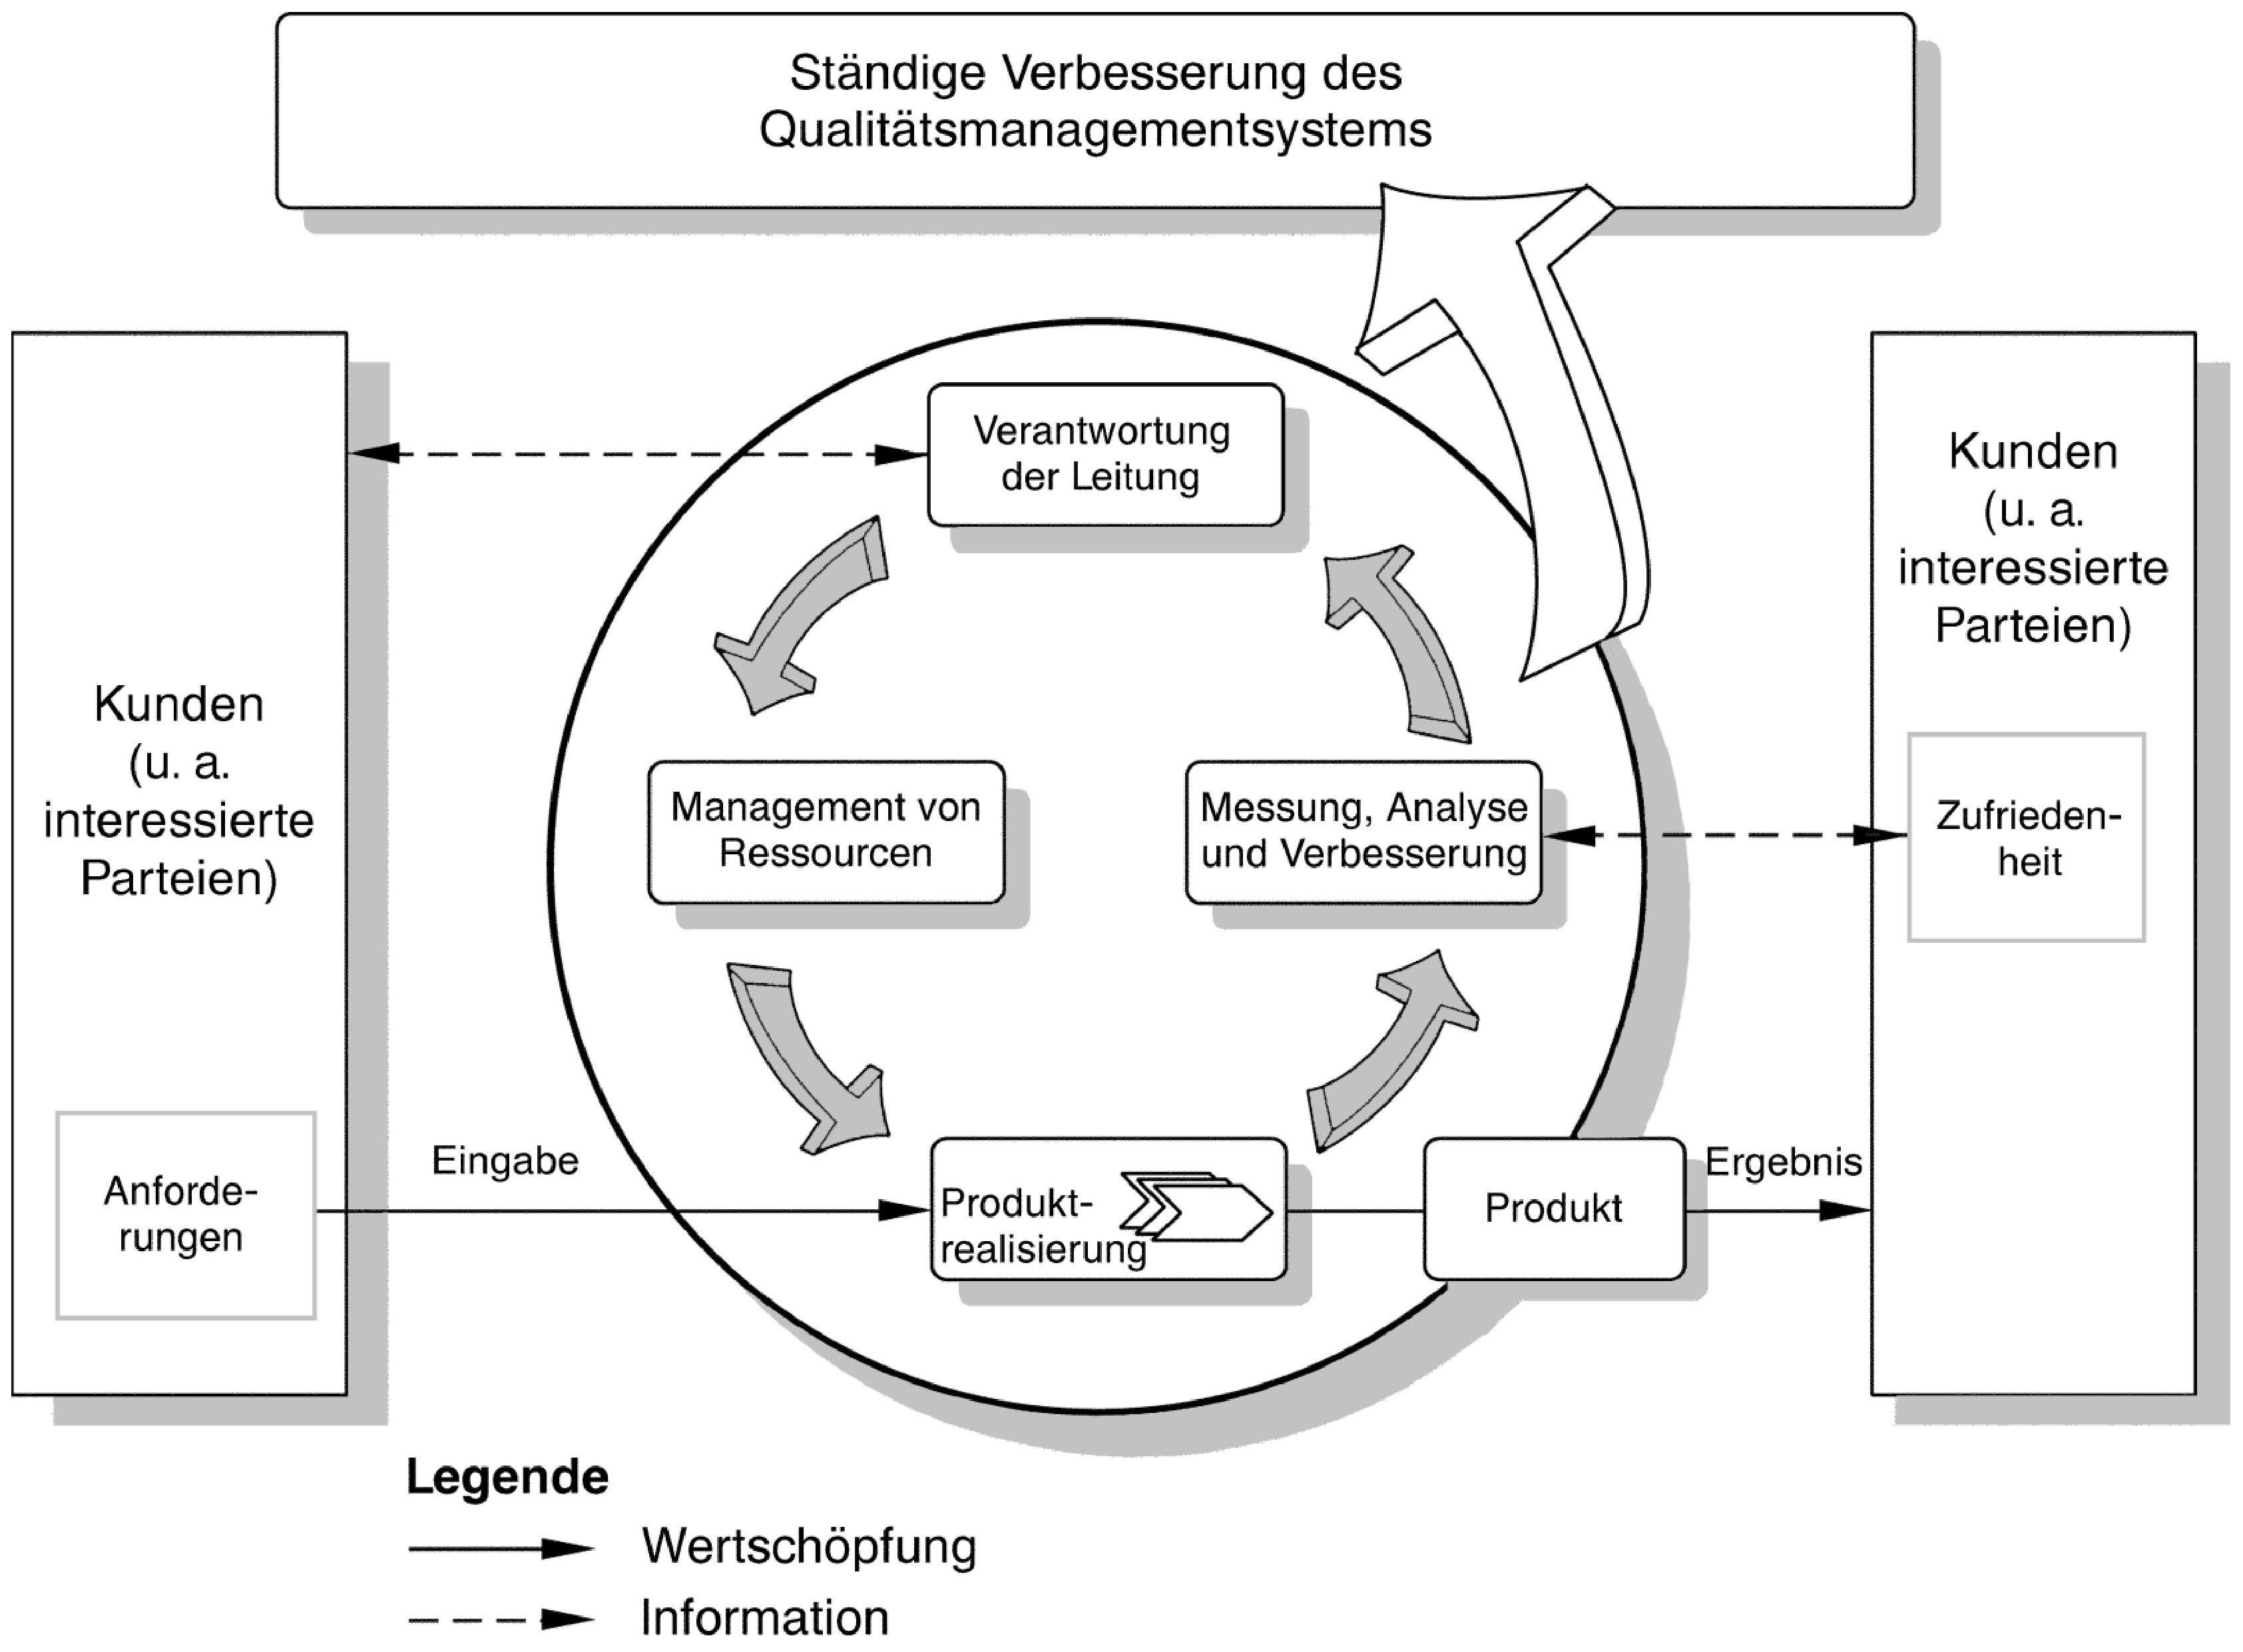
\includegraphics[width=0.7\textwidth]{../images/qm-prozess}
  \caption{Prozessorientiertes Qualitätsmanagement \citep[S.~10]{din9000}.}
  \label{fig:qm-prozess}
\end{figure}

\subsection{DIN EN ISO 9001} \label{subsec:din9001}
Möchte sich eine Organisation bzw. ein Unternehmen stärker an ihren Kunden
orientieren bzw. belegen, dass die angebotenen Produkte den Kunden- bzw.
behördlichen Anforderungen entsprechen, so kann zu diesem Zwecke ein QMS
eingeführt werden. Die ISO 9001-Norm legt die Anforderungen an ein solches QMS
fest und beschreibt dessen modellhaften Aufbau \citep{din9001}.

Eine Zertifizierung nach ISO 9001:2000 ist inzwischen weltweit anerkannt und 
gilt in vielen Bereichen als Stand der Technik. Ebenso verlangen viele 
Unternehmen von ihren Lieferanten eine solche Zertifizierung.

\subsection{DIN EN ISO 9004}
Mit dieser Norm wird ein Leitfaden bereitgestellt, der sich mit Wirksamkeit und 
der Effizienz des eingeführten QMS befasst. Insgesamt soll durch die in dieser 
Norm vorgestellten Techniken die Wirksamkeit der Organisation sowie nicht 
zuletzt die Kundenzufriedenheit gesteigert werden \citep{din9004}.